\documentclass[12pt]{article}
\usepackage{preamble}

\begin{document}
\pagenumbering{Alph}


%%%%%%%%%%%%%%%%%%%%%%%%%%%%%%%%%%%%%%%%%%%%%%%%%%%%%
%%%%%%%%%%%%%%%%%%%%% Portada %%%%%%%%%%%%%%%%%%%%%%%
%%%%%%%%%%%%%%%%%%%%%%%%%%%%%%%%%%%%%%%%%%%%%%%%%%%%%

\begin{titlepage}


	% --- LOGOTIPOS (ALINEADOS ARRIBA, IZQUIERDA Y DERECHA) ---
	\noindent
	
\includegraphics[width=0.35\textwidth]{Figuras/ule.jpg}
	\hfill
	
\includegraphics[height=2.5cm]{Figuras/escudo-ingenierias.png}

	\vspace{3cm}

	% --- BLOQUES DE TEXTO CENTRADOS ---
	\begin{center}
		{
			\fontsize{22pt}{26pt}\selectfont\bfseries
			Escuela de Ingenierías \\ Industrial, Informática y Aeroespacial
		}

		\vspace{2cm}

		{\LARGE\bfseries GRADO EN INGENIERÍA MECÁNICA} \\
		\vspace{0.5cm}
		{\LARGE\bfseries INSTALACIONES II}

		\vspace{1.5cm}

		{\Large ANÁLISIS DE PROYECTO DE APROVECHAMIENTO SOLAR PARA GENERAR AGUA CALIENTE}\\[2cm]
	\end{center}

	\vfill

	% --- AUTORES Y TUTOR (ALINEADOS A LA DERECHA) ---
	\begin{flushright}
		\large
		\begin{tabular}{@{}l@{ }l}
			\textbf{Autores:} & Alberto España Carrete    \\
			                  & Carlos Fernández Palanca  \\
			                  & Rubén Modino López        \\
			                  & Juan Diego Niño González  \\ [5pt]
			\textbf{Tutor:}   & Roberto Getino de la Mano
		\end{tabular}
	\end{flushright}

	\vspace{1.5cm}

	% --- FECHA (CENTRADA Y CON TAMAÑO ESPECÍFICO DE 22pt) ---
	\begin{center}
		{\fontsize{22pt}{26pt}\selectfont (Junio, 2026)}
	\end{center}

	\thispagestyle{empty}
\end{titlepage}

%%%% Indices -----------------------------------------------

\hypersetup{linkcolor=black}
\pagenumbering{roman}
\tableofcontents\thispagestyle{empty}

{
	\let\oldnumberline\numberline	% Añade Figura 1.1 en lugar de 1.1
	\renewcommand{\numberline}{\figurename~\oldnumberline}
	\cleardoublepage						% En pagina nueva
	\listoffigures\thispagestyle{empty}	% Pone el encabezado y pie
	\phantomsection
	\addcontentsline{toc}{section}{\listfigurename}	%Lo añade al indice

}

{
	\let\oldnumberline\numberline	% Añade Tabla 1.1 en lugar de 1.1
	\renewcommand{\numberline}{\tablename~\oldnumberline}
	\cleardoublepage		% En pagina nueva
	\listoftables\thispagestyle{empty}	% Pone el encabezado y pie
	\phantomsection
	\addcontentsline{toc}{section}{\listtablename}%Lo añade al indice
}

% En el encabezado se modifican aspectos gen. del indice.

\hypersetup{
	linkcolor=blue,
	citecolor=blue,
	urlcolor=blue
}


%%%%%%%%%%%%%%%%%%%%%%%%%%%%%%%%%%%%%%%%%%%%%%%%%%%%%%%
%%%%%%%%%%%%%%%%%%%%% Contenido %%%%%%%%%%%%%%%%%%%%%%%
%%%%%%%%%%%%%%%%%%%%%%%%%%%%%%%%%%%%%%%%%%%%%%%%%%%%%%%
\clearpage
\pagenumbering{arabic}
\section{Antecedentes y datos de partida}
\label{sec:introduccion}

\subsection{Introducción y Objetivos}
\label{subsec:origen_y_objeto}

El presente proyecto ha sido promovido a solicitud de la propiedad con el propósito de ejecutar una reforma y mejora de la eficiencia energética en un edificio residencial plurifamiliar preexistente. El objeto de la instalación consiste en definir y dimensionar un sistema solar térmico centralizado destinado a la producción de Agua Caliente Sanitaria (ACS), el cual estará hibridado con un sistema de apoyo auxiliar centralizado mediante una caldera de gas natural.

\subsection{Justificación del Sistema Centralizado}
\label{subsec:justificacion_centralizado}

\begin{itemize}
    \item \uline{Selección de Esquema:} Se adopta un esquema completamente centralizado (acumulación y apoyo centralizados en sala técnica común).
    \item \uline{Ventajas Técnicas:} 
    \begin{itemize}
        \item Simplificación de la hidráulica al interior de las viviendas y supresión de calderas individuales mixtas.
        \item Optimización del mantenimiento preventivo y correctivo al unificar los equipos de intercambio en un único espacio técnico.
        \item Liberación de superficie útil y eliminación de conductos individuales de evacuación en cada vivienda.
    \end{itemize}
    \item \uline{Criterio de Control Sanitario:} El volumen total de acumulación centralizada y la red de distribución se dimensionan para asegurar las temperaturas de consigna reglamentarias para prevenir la proliferación de microorganismos.
\end{itemize}

\subsection{Normativa de Aplicación}
\label{subsec:normativa_aplicacion}

La instalación se proyecta en estricto cumplimiento del marco reglamentario estatal vigente:

\begin{enumerate}
    \item \uline{CTE DB-HE4 (Código Técnico de la Edificación - Ahorro de Energía):} Define la contribución mínima de energía renovable para la producción de ACS en el edificio residencial \cite{cte_he4}.
    \item \uline{RITE (Reglamento de Instalaciones Térmicas en los Edificios - R.D. 1027/2007):} Establece las exigencias de eficiencia energética, seguridad y mantenimiento para la red térmica centralizada \cite{rite}.
    \item \uline{Real Decreto 487/2022:} Regula las medidas sanitarias y los requisitos de inspección y limpieza periódica física de los depósitos acumuladores de ACS para la prevención y el control de la legionelosis \cite{rd487_2022}.
    \item \uline{Real Decreto 919/2006:} Reglamento técnico de distribución y utilización de combustibles gaseosos, aplicable a la instalación del quemador de la caldera auxiliar centralizada de gas natural \cite{rd919_2006}.
    \item \uline{Norma UNE 60670:} Gobierna el diseño, ventilación, seguridad y configuración de la sala de calderas para el sistema auxiliar de gas natural en Media Presión A \cite{une60670}.
\end{enumerate}

\subsection{Ubicación Geográfica y Climatología}
\label{subsec:ubicacion_y_climatologia}

\begin{itemize}
    \item \uline{Referencia Catastral:} \texttt{5089301TL7358G0001ZD} (obtenida para el Grupo G1-1).
    \item \uline{Coordenadas Geográficas:} Latitud $40^\circ 58'\ 8.31''\text{ N}$ ($40.968975^\circ$), Longitud $5^\circ 40'\ 29.95''\text{ O}$ ($-5.674986^\circ$).
    \item \uline{Ubicación Física:} Salamanca.
\end{itemize}

La situación y el emplazamiento del edificio se recogen en el \Cref{anx:01-planos}.

En la \tabref{tab:parametros_geoclimaticos} se detallan los parámetros geoclimáticos de diseño que determinan las condiciones ambientales del proyecto.

\begin{table}[H]
\centering
\caption{Parámetros geoclimáticos de la ubicación del proyecto. Fuente: Elaboración grupal a partir de CTE DB-HE1 y CTE DB-HE4 \cite{cte_he4}.}
\label{tab:parametros_geoclimaticos}
\begin{tabularx}{\textwidth}{p{5.5cm}cX}
\toprule
\textbf{Parámetro Geoclimático} & \textbf{Valor / Clasificación} & \textbf{Origen del Dato} \\
\midrule
Zona Climática (CTE DB-HE1) & D2 & Severidad climática D (invierno), 2 (verano) \\
Zona de Radiación Solar (CTE DB-HE4) & Zona III & Irradiancia horizontal diaria media anual: $3.8 - 4.2 \text{ kWh/(m}^2\cdot\text{día)}$ \\
\bottomrule
\end{tabularx}
\end{table}

\begin{quote}
\itshape
Nota: Las coordenadas geográficas sirven exclusivamente para establecer las variables climatológicas fijas de radiación global media diaria ($H_{\text{día}}$), temperatura media ambiental ($T_{\text{amb}}$) y temperatura de entrada del agua fría de red ($T_{\text{red}}$). El azimut físico y la inclinación son parámetros geométricos independientes fijados por el diseño de la planta.
\end{quote}

\subsection{Edificación, Ocupación y Perfil de Demanda}
\label{subsec:edificacion_ocupacion_demanda}

\begin{itemize}
    \item \uline{Tipología:} Edificio residencial plurifamiliar.
    \item \uline{Número de Viviendas:} 10 viviendas de diseño estándar.
    \item \uline{Dormitorios por Vivienda:} 3 dormitorios (habitaciones) seleccionados por vivienda.
    \item \uline{Ocupación de Diseño:} 40 personas (equivalente a 4 personas por vivienda, calculadas según el estándar de ocupación del documento CTE DB-HE4 \cite{cte_he4} para viviendas de 3 dormitorios: 10 viviendas $\times$ 4 personas/vivienda).
    \item \uline{Temperatura de Referencia para ACS:} $60^\circ\text{C}$ (regulado por exigencia sanitaria antilegionella \cite{rd487_2022}).
    \item \uline{Demanda Diaria Unificada de ACS:} $1.064 \text{ L/día}$ a $60^\circ\text{C}$ \cite{cte_he4}.
\end{itemize}

\subsection{Condicionantes de Integración Física}
\label{subsec:condicionantes_integracion}

La configuración estructural del edificio impone los siguientes límites físicos para la distribución e implantación de los equipos:
\begin{itemize}
    \item \uline{Ubicación del Campo Solar:} Cubierta plana transitable (azotea) libre de obstáculos y sombras de edificaciones adyacentes.
    \item \uline{Trazado de Columnas Hidráulicas:} Canalización vertical de tuberías de ida y retorno del circuito primario y secundario a través del patinillo de comunicaciones común del edificio.
    \item \uline{Ubicación de Acumuladores:} Sala de máquinas/sala técnica común del edificio en planta baja, con acceso técnico dimensionado para el volteo de equipos.
\end{itemize}

\subsection{Equipamiento de Referencia y Fluidos}
\label{subsec:equipamiento_y_fluidos}

Se predefinen los siguientes equipos de catálogo comercial para el dimensionado físico del sistema:

\begin{itemize}
    \item \uline{Modelo de Colector Solar:} Viessmann Vitosol 200-FM (SV2F vertical) con protección integrada contra sobretemperaturas ThermProtect \cite{viessmann_vitosol}.
    \item \uline{Distribución del Campo Solar:} 12 colectores planos distribuidos simétricamente en 2 filas paralelas de 6 unidades.
    \item \uline{Parámetros Físicos del Colector (por unidad):}
    \begin{itemize}
        \item Superficie Bruta: $2.51\text{ m}^2$
        \item Superficie de Apertura: $2.33\text{ m}^2$
        \item Superficie de Absorción: $2.31\text{ m}^2$
    \end{itemize}
    \item \uline{Orientación e Inclinación del Soporte:}
    \begin{itemize}
        \item Inclinación ($\beta$): $60^\circ$ respecto a la horizontal (justificada para favorecer captación invernal y autolimitar la estival).
        \item Azimut ($\alpha$): $+20^\circ$ (desviación de $20^\circ$ al Oeste respecto al Sur geográfico).
    \end{itemize}
    \item \uline{Depósito Acumulador Prescrito:} Lapesa Master Inox MXV-2000 SS2B (Acero Inoxidable AISI 316 L) \cite{lapesa_master}.
    \begin{itemize}
        \item Capacidad Nominal: $2.000 \text{ L}$ (Bivalente con serpentines desmontables).
        \item Relación Volumen/Superficie de Apertura ($V/S_c$): $71.53 \text{ L/m}^2$ (Óptimo del IDAE).
        \item Serpentín Inferior (Solar): Desmontable de acero inoxidable con $3.4\text{ m}^2$ de superficie de intercambio.
        \item Serpentín Superior (Apoyo): Desmontable de acero inoxidable con $2.0\text{ m}^2$ de superficie de intercambio.
        \item Boca de Hombre Lateral: Brida con diámetro nominal BH DN400 para inspección física.
    \end{itemize}
    \item \uline{Fluido Caloportador y Régimen Hidráulico:}
    \begin{itemize}
        \item Caudal Volumétrico Específico ($q_{\text{esp}}$): $25 \text{ L/(h}\cdot\text{m}^2\text{ de absorción)}$ (Régimen Low-Flow).
        \item Caudal de Referencia de Diseño del Circuito Primario: $693 \text{ L/h}$ ($11.55 \text{ L/min}$) o $699 \text{ L/h}$ ($11.65 \text{ L/min}$).
        \item Fluido Caloportador: Mezcla de agua con propilenglicol al $30\%\text{ en volumen}$ para garantizar protección anticongelante hasta $-15^\circ\text{C}$ (temperatura de diseño para evitar heladas en Salamanca).
        \item Esquema de Retorno: Configuración en retorno invertido (sistema Tichelmann) para asegurar la igualdad de pérdida de carga y un caudal idéntico entre ambos ramales.
        \item Elementos de Circulación: Se contemplan de manera puramente conceptual e instrumental bombas de circulación para los circuitos primario y secundario, cuya función es permitir el transporte del fluido caloportador entre la cubierta, el interacumulador de sala técnica y la caldera de apoyo, posponiéndose su dimensionamiento hidráulico específico y la determinación de potencias para la fase de cálculo de pérdida de carga.
    \end{itemize}
    \item \uline{Respaldo Auxiliar (Gas Natural):}
    \begin{itemize}
        \item Caldera Centralizada: Caldera mural mixta de $22\text{ kW}$ de potencia útil de diseño.
        \item Combustible: Gas Natural con Poder Calorífico Superior (PCS) normalizado de $40.68\text{ MJ/m}^3\text{(s)}$.
    \end{itemize}
\end{itemize}


\begin{figure}[H]
    \centering
    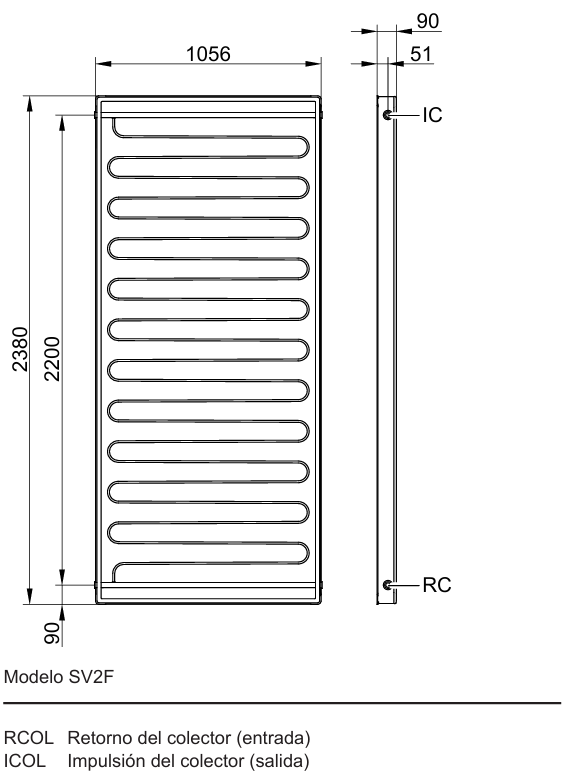
\includegraphics[width=0.7\textwidth]{Figuras/captador_seleccionado_2.png}
    \caption{Captador solar seleccionado. Fuente: Adaptado de Viessmann \cite{viessmann_vitosol}.}
    \label{fig:captador_seleccionado}
\end{figure}

\begin{figure}[H]
    \centering
    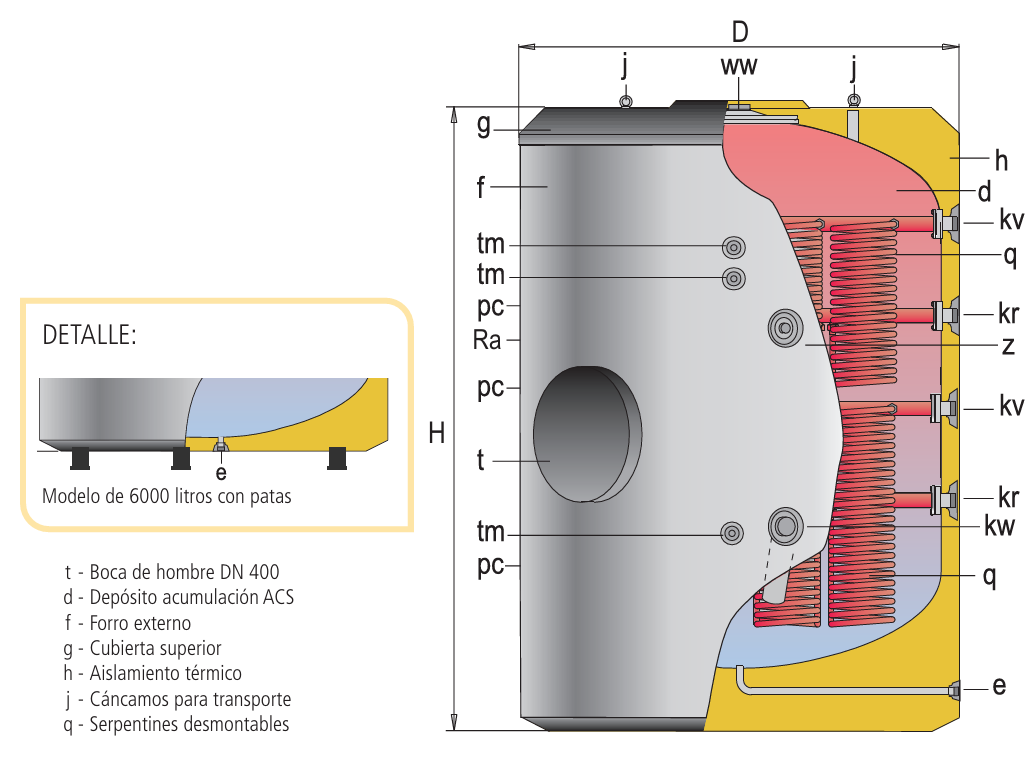
\includegraphics[width=0.55\textwidth]{Figuras/interacumulador_seleccionado.png}
    \caption{Interacumulador bivalente seleccionado. Fuente: Adaptado de Lapesa \cite{lapesa_master}.}
    \label{fig:interacumulador_seleccionado}
\end{figure}



\subsection{Balance Energético de Partida}
\label{subsec:balance_energetico_partida}

El balance energético de la instalación solar térmica permite relacionar la demanda mensual de ACS con la energía útil aportada por el campo de captadores y con la energía que debe cubrir el sistema auxiliar de gas natural. En el escenario adoptado para el proyecto se consideran 12 captadores planos, una superficie de captación de $27.96\text{ m}^2$ y un volumen de acumulación centralizada de $2.000\text{ L}$, coherente con el interacumulador bivalente seleccionado.

De forma conceptual, la energía solar incidente sobre el plano de captación se transforma en energía útil después de descontar las pérdidas ópticas y térmicas del captador, las pérdidas de transporte del circuito primario y las limitaciones asociadas al intercambio con el acumulador. Por tanto, el balance mensual puede interpretarse mediante la relación:

\begin{equation}
    Q_{\text{dem}} = Q_{\text{solar, util}} + Q_{\text{aux}}
\end{equation}

\noindent donde $Q_{\text{dem}}$ representa la demanda energética de ACS, $Q_{\text{solar, util}}$ el aporte realmente aprovechable procedente de los captadores y $Q_{\text{aux}}$ la energía complementaria suministrada por la caldera de apoyo. Esta lectura es especialmente relevante porque conecta los datos de partida de ocupación, demanda diaria, superficie de captación y volumen de acumulación con el rendimiento global esperado de la instalación.

En la \tabref{tab:balance_energetico_mensual} se recoge el balance mensual obtenido para el campo solar seleccionado. La tabla permite comparar, mes a mes, la demanda de ACS, la radiación disponible en el plano inclinado de los captadores, la fracción solar alcanzada y la energía útil realmente aportada por la instalación solar.

\begin{table}[H]
\centering
\caption{Balance energético mensual de la instalación solar térmica. Fuente: Elaboración grupal a partir de la hoja de cálculo del proyecto.}
\label{tab:balance_energetico_mensual}
\begin{tabular}{lrrrr}
\toprule
\textbf{Mes} & \textbf{Demanda ACS} & \textbf{Radiación incl.} & \textbf{Fracción solar} & \textbf{Energía útil} \\
 & \textbf{(kWh)} & \textbf{(kWh/m$^2$)} & \textbf{(\%)} & \textbf{(kWh)} \\
\midrule
Enero & 2.104 & 73,03 & 43 & 899 \\
Febrero & 1.866 & 91,80 & 62 & 1.151 \\
Marzo & 1.990 & 123,79 & 76 & 1.506 \\
Abril & 1.851 & 127,86 & 81 & 1.499 \\
Mayo & 1.875 & 130,47 & 82 & 1.546 \\
Junio & 1.777 & 136,76 & 90 & 1.602 \\
Julio & 1.798 & 162,92 & 101 & 1.798 \\
Agosto & 1.837 & 176,54 & 106 & 1.837 \\
Septiembre & 1.814 & 163,92 & 102 & 1.814 \\
Octubre & 1.913 & 133,36 & 83 & 1.583 \\
Noviembre & 1.925 & 94,85 & 60 & 1.161 \\
Diciembre & 2.104 & 67,99 & 39 & 823 \\
\midrule
\textbf{Anual} & \textbf{22.856} & -- & \textbf{75,3} & \textbf{17.219} \\
\bottomrule
\end{tabular}
\end{table}

El resultado anual obtenido proporciona una fracción solar del $75,3\%$, superior a la exigencia mínima considerada en la hoja de cálculo. La lectura de la \tabref{tab:balance_energetico_mensual} muestra tres comportamientos diferenciados. En primer lugar, diciembre y enero son los meses más desfavorables, con fracciones solares del $39\%$ y del $43\%$ respectivamente; en ellos la demanda alcanza $2.104\text{ kWh}$ y el aporte solar útil queda limitado a $823\text{ kWh}$ y $899\text{ kWh}$, por lo que el respaldo auxiliar resulta imprescindible. En segundo lugar, de marzo a junio y en octubre la cobertura solar se mantiene elevada pero controlada, entre el $76\%$ y el $90\%$, lo que representa el rango de funcionamiento más equilibrado de la instalación. Finalmente, julio, agosto y septiembre superan ligeramente el $100\%$ de fracción mensual; el caso más exigente es agosto, con un $106\%$, sin rebasar el límite de sobreproducción mensual del $110\%$.

\begin{figure}[H]
    \centering
    \includegraphics[width=\textwidth, trim={2cm 3cm 1.5cm 3.5cm},clip=true]{Figuras/balance_energetico.pdf}
    \caption{Balance energético mensual de la instalación solar térmica para ACS. Fuente: Elaboración grupal a partir de la hoja de cálculo del proyecto.}
    \label{fig:balance_energetico_solar_termica}
\end{figure}

Como se observa en la \figref{fig:balance_energetico_solar_termica}, el aporte solar útil reduce de forma significativa la energía auxiliar necesaria durante la mayor parte del año, pero no elimina la necesidad del respaldo centralizado. Por este motivo, el balance energético justifica simultáneamente la superficie de captadores adoptada, el volumen de acumulación de $2.000\text{ L}$ y la presencia de la caldera auxiliar para garantizar la continuidad del servicio en los meses de menor radiación.


\section{Cálculos}
\label{sec:calculos}

En este apartado se desarrollan las comprobaciones y los dimensionamientos hidráulicos de los circuitos principales que integran la instalación solar térmica con soporte auxiliar de gas natural: el circuito primario solar, el circuito secundario (analizado a través de las conexiones de llenado y acometida), la red de distribución y recirculación de agua caliente sanitaria (ACS), y la selección unificada de las bombas de circulación Grundfos. Todas las comprobaciones se fundamentan en los datos meteorológicos específicos de la zona y en los requerimientos sanitarios vigentes para garantizar una instalación segura, higiénica y energéticamente eficiente.

\subsection{Circuito primario solar}
\label{subsec:circuito_primario_solar}

El circuito primario solar está constituido por un bucle hidráulico cerrado ubicado en la azotea del edificio que transporta el fluido caloportador desde el campo de captadores hasta el intercambiador de calor integrado en el acumulador centralizado. Para garantizar la operatividad de la instalación frente a las heladas en Salamanca (zona climática D2), se prescribe como fluido caloportador una mezcla de agua con anticongelante de tipo propilenglicol atóxico con una concentración en volumen comprendida entre el 30\% y el 50\%, la cual evita la congelación en invierno y protege el circuito contra la corrosión y la degradación por altas temperaturas.

El campo solar consta de 12 captadores solares planos Viessmann Vitosol 200-FM SV2F instalados en disposición vertical, lo que proporciona una superficie de apertura unitaria de $2,33\text{ m}^2$ y una superficie de apertura total de:
\begin{equation}
    S_{\text{apertura}} = 12 \times 2,33\text{ m}^2 = 27,96\text{ m}^2
\end{equation}
Para asegurar un reparto equilibrado del caudal y minimizar la pérdida de carga global, el campo de captadores se divide en dos baterías paralelas de 6 captadores (denominadas C1 y C2) conectadas bajo el esquema de retorno invertido (red de Tichelmann). 

El caudal total de diseño del primario en régimen de bajo caudal (\textit{low-flow}) es de $699\text{ l/h}$. Debido a la simetría geométrica y de pérdidas del retorno invertido, el caudal se divide por igual entre ambos ramales, correspondiendo un caudal de diseño por batería de $349,5\text{ l/h}$:
\begin{equation}
    Q_{\text{ramal}} = \frac{699\text{ l/h}}{2} = 349,5\text{ l/h}
\end{equation}
Las tuberías de cobre se dimensionan en consecuencia, prescribiendo un diámetro exterior de DN22 (diámetro interior de $20\text{ mm}$) para los tramos comunes entre el depósito y la bifurcación, y un diámetro exterior de DN18 (diámetro interior de $16\text{ mm}$) para las ramas individuales de las baterías C1 y C2.

Para la determinación del punto de trabajo mínimo del circulador, se calcula la pérdida de carga del recorrido hidráulico críticamente desfavorable, correspondiente al ramal C1. Las pérdidas de carga dinámicas en el primario son:
\begin{itemize}
    \item Pérdidas dinámicas de carga por fricción y accesorios en las tuberías del tramo más desfavorable: $0,534\text{ m.c.a.}$
    \item Pérdida de carga interna en el lado primario del intercambiador de calor del depósito acumulador: $1,50\text{ m.c.a.}$
    \item Pérdida de carga agregada en el campo de captadores, considerando que el fluido atraviesa una batería de 6 captadores con una pérdida de carga unitaria de $30\text{ mm.c.a.}$ por captador:
    \begin{equation}
        P_{\text{dc, captadores}} = 6 \times 30\text{ mm.c.a.} = 180\text{ mm.c.a.} = 0,18\text{ m.c.a.}
    \end{equation}
\end{itemize}
La pérdida de carga dinámica total del circuito primario solar resulta de la suma de las pérdidas de tuberías, intercambiador y captadores:
\begin{equation}
    P_{\text{dc, total}} = 0,534\text{ m.c.a.} + 1,50\text{ m.c.a.} + 0,18\text{ m.c.a.} = 2,214\text{ m.c.a.}
\end{equation}
Por tanto, la bomba del primario se dimensionará para satisfacer un punto de trabajo de diseño de $699\text{ l/h}$ de caudal a una altura manométrica mínima de $2,21\text{ m.c.a.}$

El volumen total de fluido del circuito primario se determina sumando los volúmenes interiores de las tuberías de ida y retorno ($5,22\text{ l}$), del campo de captadores ($21,96\text{ l}$) y del serpentín primario del interacumulador ($20\text{ l}$):
\begin{equation}
    V_{\text{total}} = 5,22\text{ l} + 21,96\text{ l} + 20\text{ l} = 47,18\text{ l}
\end{equation}
A partir de este volumen de fluido y aplicando un coeficiente de dilatación de $0,08$ (para mezclas con anticongelante y temperaturas de trabajo elevadas), una presión inicial de llenado en frío de $1,5\text{ kg/cm}^2$ y una presión final de tarado de la válvula de seguridad de $4\text{ kg/cm}^2$, se calcula un volumen del vaso de expansión de aproximadamente $6\text{ l}$. Con fines de seguridad frente a dilataciones extremas, se prescribe un modelo comercial estándar de \textbf{8 l} de capacidad.

Al final de esta subsección, en la \tabref{tab:pdc_primario}, se recoge el desglose detallado del cálculo de pérdidas de carga por tramo en el circuito primario.

\begin{landscape}
\begin{table}[p]
\centering
\footnotesize
\setlength{\tabcolsep}{2pt}
\caption{Pérdidas de carga detalladas por tramo en el circuito primario solar. Fuente: Elaboración grupal.}
\label{tab:pdc_primario}
\begin{tabular}{llccccccccccrccc}
\toprule
\textbf{Tramo} & \textbf{Desf.} & \textbf{Caudal} & \textbf{DN} & \textbf{Di} & \textbf{Velocidad} & \textbf{Pdc lin.} & \textbf{Espesor} & \textbf{L recto} & \textbf{Sing. 1} & \textbf{N.º} & \textbf{Sing. 2} & \textbf{N.º} & \textbf{L eq. sing.} & \textbf{L total} & \textbf{Pdc} \\
 & & \textbf{(l/h)} & \textbf{(mm)} & \textbf{(mm)} & \textbf{(m/s)} & \textbf{(mm.c.a./m)} & \textbf{aisl. (mm)} & \textbf{(m)} & & & & & \textbf{(m)} & \textbf{(m)} & \textbf{(mm.c.a.)} \\
\midrule
C1-A & Sí & 349,5 & 18 & 16 & 0,48 & 26,5 & 30 & 6,06 & Codo 90º & 1 & Te tipo 2 & 1 & 3,00 & 9,06 & 239,9 \\
C2-A & No & 349,5 & 18 & 16 & 0,48 & 26,5 & 30 & 1,03 & Te tipo 1 & 1 & --- & & 0,15 & 1,18 & 31,2 \\
A-Depósito & No & 699 & 22 & 20 & 0,62 & 30,9 & 30 & 3,78 & Te tipo 1 & 1 & --- & & 0,20 & 3,98 & 122,8 \\
Depósito-B & No & 699 & 22 & 20 & 0,62 & 30,9 & 30 & 3,65 & Te tipo 1 & 1 & --- & & 0,20 & 3,85 & 118,8 \\
B-C2 & No & 349,5 & 18 & 16 & 0,48 & 26,5 & 30 & 1,34 & Te tipo 1 & 1 & --- & & 0,15 & 1,49 & 39,5 \\
B-C1 & No & 349,5 & 18 & 16 & 0,48 & 26,5 & 30 & 6,82 & Codo 90º & 1 & Te tipo 1 & 1 & 0,65 & 7,47 & 197,8 \\
\bottomrule
\end{tabular}
\end{table}
\end{landscape}

\subsection{Circuito secundario solar}
\label{subsec:circuito_secundario_solar}

El circuito secundario solar tiene como objetivo captar la energía transmitida por el circuito primario y acumularla térmicamente en el agua sanitaria destinada al consumo. En este diseño se adopta un interacumulador centralizado bivalente de $2.000\text{ l}$ de capacidad (modelo Lapesa Master Inox MXV-2000 SS2B) provisto de un serpentín inferior interno desmontable. De este modo, la transferencia de energía solar se realiza de forma estática directamente al agua potable almacenada en la cuba. Al no existir un intercambiador de placas externo, se prescinde de un circuito hidráulico cerrado y de una bomba de circulación para el secundario solar.

Para documentar y verificar la red hidráulica en la sala técnica de la azotea, se evalúan las comprobaciones hidráulicas correspondientes a las conexiones de entrada de agua sanitaria desde la acometida de red al depósito y de este a la base de la bajante general del edificio:
\begin{itemize}
    \item Caudal de diseño del secundario: Se determina mediante la aplicación de un caudal de diseño de $50\text{ l/(h}\cdot\text{m}^2)$ sobre la superficie de apertura del campo solar de $27,96\text{ m}^2$, resultando un caudal de $1.398\text{ l/h}$.
    \begin{equation}
        Q_{\text{secundario}} = 27,96\text{ m}^2 \times 50\text{ l/(h}\cdot\text{m}^2) = 1.398\text{ l/h}
    \end{equation}
    \item Dimensionado de tuberías: Para la conducción de este caudal se adopta un diámetro exterior de DN28 en cobre (diámetro interior de $26\text{ mm}$), lo que permite que el agua circule a una velocidad de $0,73\text{ m/s}$.
    \item Pérdidas de carga: Sumando las pérdidas dinámicas en tuberías y accesorios ($0,63\text{ m.c.a.}$) and las pérdidas internas del secundario en el serpentín intercambiador inferior del acumulador ($1,30\text{ m.c.a.}$), la pérdida de carga hidráulica de conexión es de:
    \begin{equation}
        P_{\text{dc, conexión}} = 0,63\text{ m.c.a.} + 1,30\text{ m.c.a.} = 1,93\text{ m.c.a.}
    \end{equation}
    \item Potencia mínima del intercambiador: Para evitar retenciones en la transferencia térmica, se aplica un criterio de potencia mínima de intercambio de $600\text{ W}$ por cada metro cuadrado de superficie de apertura de captación. Esto impone una potencia mínima de diseño del serpentín de:
    \begin{equation}
        P_{\text{mín}} = 27,96\text{ m}^2 \times 600\text{ W/m}^2 = 16.776\text{ W} = 16,8\text{ kW}
    \end{equation}
    Dicha exigencia queda satisfecha por los $3,4\text{ m}^2$ de superficie de intercambio del serpentín inferior del interacumulador Lapesa seleccionado.
\end{itemize}

En la \tabref{tab:pdc_secundario} se desglosa el cálculo de pérdidas de carga.
\begin{landscape}
\begin{table}[p]
\centering
\footnotesize
\setlength{\tabcolsep}{2pt}
\caption{Pérdidas de carga por tramo en las conexiones hidráulicas sanitarias del circuito secundario solar. Fuente: Elaboración grupal.}
\label{tab:pdc_secundario}
\begin{tabular}{lccccccclcccc}
\toprule
\textbf{Tramo} & \textbf{Caudal} & \textbf{DN} & \textbf{Di} & \textbf{Velocidad} & \textbf{Pdc lin.} & \textbf{Espesor} & \textbf{L recto} & \textbf{Sing. 1} & \textbf{N.º} & \textbf{L eq. sing.} & \textbf{L total} & \textbf{Pdc} \\
 & \textbf{(l/h)} & \textbf{(mm)} & \textbf{(mm)} & \textbf{(m/s)} & \textbf{(mm.c.a./m)} & \textbf{aisl. (mm)} & \textbf{(m)} & & & \textbf{(m)} & \textbf{(m)} & \textbf{(mm.c.a.)} \\
\midrule
Red-Depósito & 1.398 & 28 & 26,0 & 0,73 & 23,0 & 20 & 17,00 & Codo 90º & 2 & 1,52 & 18,52 & 425,3 \\
Depósito-Bajante & 1.398 & 28 & 26,0 & 0,73 & 23,0 & 20 & 6,58 & Codo 90º & 3 & 2,28 & 8,86 & 203,4 \\
\bottomrule
\end{tabular}
\end{table}
\end{landscape}

\subsection{Circuito de distribución de ACS}
\label{subsec:circuito_distribucion_acs}

El circuito de distribución de ACS conduce el agua potable sanitaria precalentada desde la sala técnica en azotea hasta la entrada de las calderas murales mixtas individuales situadas en cada una de las 10 viviendas del edificio (distribuidas en 5 plantas con 2 viviendas por planta).

El caudal equivalente unificado para cada vivienda se establece en $0,25\text{ l/s}$ ($900\text{ l/h}$), representativo del caudal de entrada a la caldera individual. A lo largo de la bajante vertical principal, que discurre por el patio interior del edificio, el caudal de diseño acumulado decrece progresivamente a medida que se derivan las tomas de cada planta. Aplicando los correspondientes coeficientes de simultaneidad y criterios de velocidad admisible, el diámetro exterior de la bajante se reduce de forma escalonada de DN42 en el tramo común superior (donde alimenta las 10 viviendas con un caudal máximo simultáneo de $2,50\text{ l/s}$) a DN22 en el tramo de alimentación final inferior (P2-P1). Las derivaciones individuales desde la bajante general a la caldera de cada vivienda se dimensionan con una tubería de cobre DN18.

Para dar cumplimiento al Real Decreto 487/2022 de prevención de legionelosis, la red se complementa con una tubería de recirculación de ACS de retorno que discurre en sentido ascendente desde el extremo inferior de la bajante hasta el depósito acumulador. Este retorno garantiza que el agua sanitaria se mantenga a una temperatura superior a los $50^\circ\text{C}$ en las derivaciones de consumo durante períodos de inactividad, evitando el estancamiento y enfriamiento del agua. Para esta red de retorno de recirculación, se establece un caudal de recirculación de diseño de $360\text{ l/h}$ ($0,10\text{ l/s}$) and una tubería DN18 (diámetro interior de $16\text{ mm}$), que con una longitud total de 17 m genera una velocidad de flujo de $0,50\text{ m/s}$ y una pérdida de carga dinámica de $0,36\text{ m.c.a.}$.

En la \tabref{tab:tramos_distribucion} se desglosa el dimensionamiento de los tramos de impulsión de la bajante de ACS y el retorno de recirculación.

\begin{landscape}
\begin{table}[p]
\centering
\footnotesize
\setlength{\tabcolsep}{2pt}
\caption{Dimensionado hidráulico y pérdidas térmicas por tramo en la bajante e impulsión de ACS y retorno de recirculación. Fuente: Elaboración grupal.}
\label{tab:tramos_distribucion}
\begin{tabular}{lcccccccccccc}
\toprule
\textbf{Tramo} & \textbf{Recirc.} & \textbf{n viv} & \textbf{Coef.} & \textbf{Caudal} & \textbf{Caudal} & \textbf{DN} & \textbf{Di} & \textbf{Velocidad} & \textbf{Espesor} & \textbf{Pérdidas} & \textbf{L recto} & \textbf{Pérdidas} \\
 & & & \textbf{simult.} & \textbf{(l/s)} & \textbf{(l/h)} & \textbf{(mm)} & \textbf{(mm)} & \textbf{(m/s)} & \textbf{aisl. (mm)} & \textbf{(W/m)} & \textbf{(m)} & \textbf{(W)} \\
\midrule
Bajante-P5 & No & 10 & 0,45 & 2,50 & 9.000 & 42 & 40 & 1,99 & 30 & 12,9 & 2,60 & 33,54 \\
P5-V10 & No & 1 & 1,00 & 0,25 & 900 & 18 & 16 & 1,24 & 20 & 7,5 & 5,65 & 42,375 \\
P5-V9 & No & 1 & 1,00 & 0,25 & 900 & 18 & 16 & 1,24 & 20 & 7,5 & 5,65 & 42,375 \\
P5-P4 & No & 8 & 0,48 & 2,00 & 7.200 & 42 & 40 & 1,59 & 30 & 12,9 & 2,60 & 33,54 \\
P4-V8 & No & 1 & 1,00 & 0,25 & 900 & 18 & 16 & 1,24 & 20 & 7,5 & 5,65 & 42,375 \\
P4-V7 & No & 1 & 1,00 & 0,25 & 900 & 18 & 16 & 1,24 & 20 & 7,5 & 5,65 & 42,375 \\
P4-P3 & No & 6 & 0,50 & 1,50 & 5.400 & 35 & 33 & 1,76 & 20 & 11,4 & 2,60 & 29,64 \\
P3-V6 & No & 1 & 0 & 0,25 & 900 & 18 & 16 & 1,24 & 20 & 7,5 & 5,65 & 42,375 \\
P3-V5 & No & 1 & 0 & 0,25 & 900 & 18 & 16 & 1,24 & 20 & 7,5 & 5,65 & 42,375 \\
P3-P2 & No & 4 & 0 & 1,00 & 3.600 & 28 & 26 & 1,89 & 20 & 9,8 & 2,60 & 25,48 \\
P2-V4 & No & 1 & 0 & 0,25 & 900 & 18 & 16 & 1,24 & 20 & 7,5 & 5,65 & 42,375 \\
P2-V3 & No & 1 & 0 & 0,25 & 900 & 18 & 16 & 1,24 & 20 & 7,5 & 5,65 & 42,375 \\
P2-P1 & No & 2 & 0 & 0,50 & 1.800 & 22 & 20 & 1,59 & 20 & 8,4 & 2,60 & 21,84 \\
P1-V2 & No & 1 & 0 & 0,25 & 900 & 18 & 16 & 1,24 & 20 & 7,5 & 5,65 & 42,375 \\
P1-V1 & No & 1 & 0 & 0,25 & 900 & 18 & 16 & 1,24 & 20 & 7,5 & 5,65 & 42,375 \\
P1-Depósito & Sí & 0 & 0 & 0 & 0 & 18 & 16 & 0 & 20 & 7,5 & 17,00 & 127,50 \\
\bottomrule
\end{tabular}
\end{table}
\end{landscape}

\subsection{Selección de bombas}
\label{subsec:seleccion_de_bombas}

Para asegurar la máxima compatibilidad operativa, facilidad de mantenimiento e integración con los sistemas de control del edificio, se unifica la marca de los equipos de bombeo hidráulico bajo el fabricante \textbf{Grundfos}, prescribiéndose un circulador electrónico de rotor húmedo para cada una de las dos aplicaciones requeridas.

\paragraph{Bomba del Circuito Primario Solar (ALPHA SOLAR 25-75 180)}
\label{par:bomba_primario}

La bomba encargada de impulsar el fluido caloportador en el primario solar es el modelo Grundfos ALPHA SOLAR 25-75 180 (Número de Producto: 98989300) \cite{grundfos_alpha_solar}:
\begin{itemize}
    \item \textbf{Ubicación física:} Se instala en la tubería común de retorno frío en la cubierta (azotea) del edificio, aguas abajo de la salida del serpentín del interacumulador Lapesa y antes del campo de captadores.
    \item \textbf{Justificación de la ubicación y montaje:}
    \begin{enumerate}
        \item \textit{Protección frente a temperatura:} En la zona de retorno, el fluido caloportador se encuentra a menor temperatura que en la ida, lo que evita que las juntas elastómeras, los cojinetes y el módulo electrónico estén sometidos de forma continua a las altas temperaturas de impulsión ($>95^\circ\text{C}$).
        \item \textit{Evitación de cavitación:} La temperatura de retorno reduce la presión de vaporización del fluido caloportador y eleva la presión neta de aspiración positiva (NPSH disponible) a la entrada de la bomba, previniendo la cavitación.
        \item \textit{Alineación del eje:} Por requerimientos mecánicos del fabricante, la bomba se debe instalar obligatoriamente con el eje del rotor en posición horizontal para garantizar la adecuada lubricación de sus cojinetes y favorecer la purga natural del aire del circuito.
        \item \textit{Bucle cerrado:} El circuito primario solar opera como una tubería cerrada sobre la cubierta, de forma que el peso de las columnas vertical ascendente y descendente del bucle se compensa hidrostáticamente. El circulador no debe vencer cota estática de elevación del agua y sus requerimientos mecánicos responden de manera exclusiva a las pérdidas de carga dinámicas de fricción, calculadas en $2,21\text{ m.c.a.}$ para el caudal de diseño de $699\text{ l/h}$. La bomba seleccionada cuenta con una altura nominal máxima de $7,5\text{ m.c.a.}$, cubriendo este requerimiento con óptima eficiencia energética.
    \end{enumerate}
    \item \textbf{Regulación y conexiones:} La regulación de la velocidad se realiza mediante una señal electrónica externa de modulación de ancho de pulso PWM (Perfil C) enviada desde el controlador de la instalación solar colectiva. Su conexión hidráulica se realiza mediante rosca G 1 1/2'' (DN25) utilizando racores de unión rosca-soldar 1 1/2'' a 22 mm para la acoplación directa a la tubería de cobre DN22 común.
\end{itemize}

En la \figref{fig:bomba_primario} se muestra el circulador Grundfos ALPHA SOLAR seleccionado.

\begin{figure}[H]
    \centering
    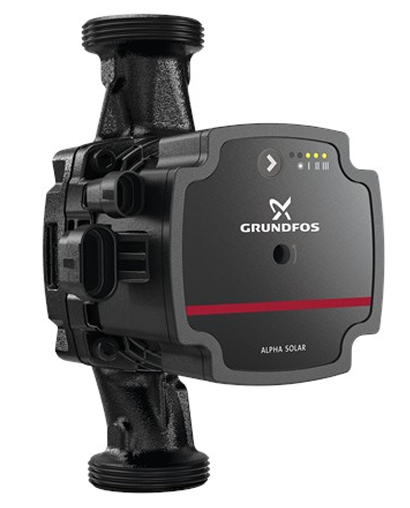
\includegraphics[width=0.45\textwidth]{Figuras/bomba_circuito_primario.png}
    \caption{Bomba de circulación electrónica de alta eficiencia Grundfos ALPHA SOLAR 25-75 180. Fuente: Adaptado de Grundfos \cite{grundfos_alpha_solar}.}
    \label{fig:bomba_primario}
\end{figure}

\paragraph{Bomba de Recirculación de ACS (ALPHA2 25-40 N 180)}
\label{par:bomba_recirculacion}

La bomba encargada de mantener el caudal en el anillo de recirculación sanitaria es el modelo Grundfos ALPHA2 25-40 N 180 (Número de Producto: 99411365) \cite{grundfos_alpha2}:
\begin{itemize}
    \item \textbf{Ubicación física:} Se coloca en la tubería del retorno de recirculación en la cubierta (sala técnica), inmediatamente antes de su conexión al interacumulador Lapesa.
    \item \textbf{Justificación de la selección y seguridad sanitaria:}
    \begin{enumerate}
        \item \textit{Material higiénico:} Tratándose de un circuito abierto por el que circula agua de consumo humano, es de imperativo cumplimiento normativo prescribir una bomba con cuerpo de \textbf{Acero Inoxidable (AISI 304)} para evitar fenómenos de corrosión galvánica y asegurar la calidad higiénica del agua sanitaria, motivo por el cual se prescribe el modelo con terminación ``N''.
        \item \textit{Control de recirculación:} Dispone de regulación electrónica inteligente mediante la función \textit{AUTOADAPT}, que ajusta de forma constante la velocidad del circulador en función de la demanda real del edificio. Esto reduce al mínimo el consumo energético (de 3 a 18 W), previene molestias por ruidos de flujo en las viviendas y evita la erosión de las tuberías de cobre de DN18.
        \item \textit{Márgenes de seguridad hidráulica:} A partir del caudal calculado de $360\text{ l/h}$ y la pérdida de carga teórica del retorno de $0,36\text{ m.c.a.}$, se aplica un margen del 15\% en caudal (caudal de diseño de $425\text{ l/h}$ para asegurar la uniformidad térmica en el extremo de la red) y un margen del 50\% al 100\% en presión manométrica (altura de diseño de $0,6$ a $0,8\text{ m.c.a.}$). Este amplio margen de presión se justifica para compensar la pérdida de carga singular de la válvula de retención obligatoria a la salida (que impide flujos inversos desde la red), del filtro de impurezas obligatorio a la entrada (que protege el rotor frente a cal y partículas) y el previsible aumento de la rugosidad de la tubería debido al envejecimiento y las incrustaciones a largo plazo. Con una altura máxima de diseño de $H_{\text{max}} = 4,0\text{ m.c.a.}$, la bomba proporciona una reserva hidráulica idónea.
    \end{enumerate}
\end{itemize}

En la \figref{fig:bomba_recirculacion} se ilustra el circulador Grundfos ALPHA2 en acero inoxidable.

\begin{figure}[H]
    \centering
    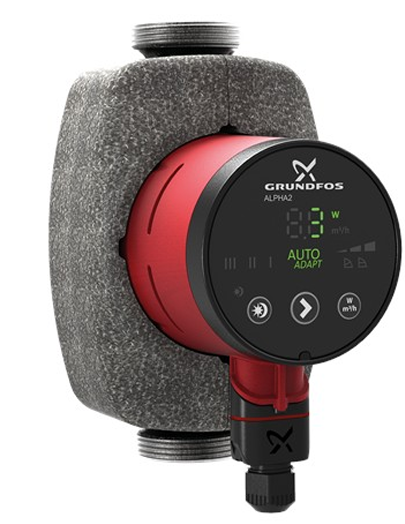
\includegraphics[width=0.45\textwidth]{Figuras/bomba_recirculacion.png}
    \caption{Bomba de recirculación de ACS en acero inoxidable Grundfos ALPHA2 25-40 N 180. Fuente: Adaptado de Grundfos \cite{grundfos_alpha2}.}
    \label{fig:bomba_recirculacion}
\end{figure}

Los datos técnicos de ambos equipos de bombeo, se presenta en la \tabref{tab:especificaciones_bombas}.

\begin{table}[H]
\centering
\caption{Matriz unificada de especificaciones de las bombas de circulación Grundfos. Fuente: Adaptado de Grundfos \cite{grundfos_alpha_solar, grundfos_alpha2}.}
\label{tab:especificaciones_bombas}
\begin{tabularx}{\textwidth}{lXX}
\toprule
\textbf{Variable de Selección} & \textbf{Bomba Primario Solar (ALPHA SOLAR)} & \textbf{Bomba Recirculación ACS (ALPHA2 N)} \\
\midrule
Modelo Prescrito & Grundfos ALPHA SOLAR 25-75 180 & Grundfos ALPHA2 25-40 N 180 \\
Número de Producto & 98989300 & 99411365 \\
Material del Cuerpo & Fundición de Hierro (Cataforesis) & Acero Inoxidable (AISI 304) \\
Altura Nominal Máxima & $7,5\text{ m.c.a.}$ & $4,0\text{ m.c.a.}$ \\
Caudal Máximo & $3,5\text{ m}^3\text{/h}$ & $2,4\text{ m}^3\text{/h}$ \\
Fluido de Trabajo & Agua + Glicol Propileno (30-50\%) & Agua Potable Sanitaria \\
Rango de Temperatura & $2^\circ\text{C}$ a $110^\circ\text{C}$ & $2^\circ\text{C}$ a $110^\circ\text{C}$ \\
Tipo de Conexión & Rosca G 1 1/2'' & Rosca G 1 1/2'' (DN25) \\
Longitud entre Bocas & $180\text{ mm}$ & $180\text{ mm}$ \\
Consumo Eléctrico & $2 - 45\text{ W}$ & $3 - 18\text{ W}$ \\
Índice de Eficiencia (EEI) & $\le 0,20$ & $\le 0,15$ \\
Modo de Control & PWM externo (Perfil C) / Curvas & AUTOADAPT / Presión variable \\
\bottomrule
\end{tabularx}
\end{table}

Cabe señalar de manera explícita que, dada la concepción y los límites físicos del presente proyecto residencial centralizado de ACS, no se requiere el dimensionamiento ni la especificación de circuladores adicionales para el secundario solar ni de bombas de apoyo auxiliares para la caldera en este alcance técnico.


\renewcommand{\refname}{Bibliografía}
\bibliographystyle{IEEEtran}
\cleardoublepage
\phantomsection
\addcontentsline{toc}{section}{Bibliografía}
\bibliography{refs}

\clearpage


\myappendix{Características técnicas de los equipos}

\begin{appendixspecialsections}
	\section{Captadores solares}

		\includepdf[pages=-, fitpaper=true]{Figuras/ficha_tecnica_captador_Vitosol_200-FM.pdf}



	\section{Depósito de acumulación e intercambiador de calor integrado}

		\includepdf[pages=-, fitpaper=true]{Figuras/ficha_tecnica_intercambiador_MXV-2000-SS2B.pdf}

	\section{Bombas de circulación}

		\subsection{Bomba del circuito primario (Solar)}
		\includepdf[pages=-, fitpaper=true]{Figuras/bomba_circuito_primario_ALPHA_SOLAR_25-75__180.pdf}

		\subsection{Bomba de Recirculación de ACS}
		\includepdf[pages=-, fitpaper=true]{Figuras/bomba_recirculacion_ALPHA2_2540_N_180.pdf}

\end{appendixspecialsections}


\myappendix{Planos}
\label{anx:01-planos}

\includepdf[pages=-, fitpaper=true]{Figuras/Planos/emplazamiento-situacion.pdf}
\includepdf[pages=-, fitpaper=true]{Figuras/Planos/plano_azotea.pdf}

\includepdf[pages=-, fitpaper=true]{Figuras/Planos/plano_instalacion_solar_primario_Azotea.pdf}

\includepdf[pages=-, fitpaper=true]{Figuras/Planos/plano_instalacion_distribucion.pdf}








\end{document}
